

\tikzset{every picture/.style={line width=0.75pt}} %set default line width to 0.75pt        

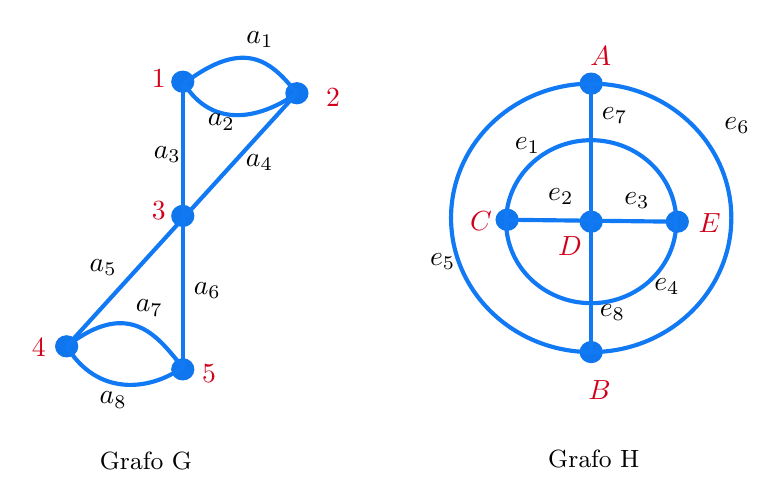
\begin{tikzpicture}[x=0.75pt,y=0.75pt,yscale=-1,xscale=1]
%uncomment if require: \path (0,238); %set diagram left start at 0, and has height of 238

%Shape: Ellipse [id:dp8399187232641918] 
\draw  [draw opacity=0][fill={rgb, 255:red, 15; green, 118; blue, 237 }  ,fill opacity=1 ] (143.36,36.95) .. controls (143.36,33.99) and (145.87,31.59) .. (148.96,31.59) .. controls (152.05,31.59) and (154.56,33.99) .. (154.56,36.95) .. controls (154.56,39.91) and (152.05,42.31) .. (148.96,42.31) .. controls (145.87,42.31) and (143.36,39.91) .. (143.36,36.95) -- cycle ;
%Shape: Ellipse [id:dp8527982659961908] 
\draw  [draw opacity=0][fill={rgb, 255:red, 15; green, 118; blue, 237 }  ,fill opacity=1 ] (88.38,169.99) .. controls (88.38,167.03) and (90.88,164.62) .. (93.98,164.62) .. controls (97.07,164.62) and (99.58,167.03) .. (99.58,169.99) .. controls (99.58,172.95) and (97.07,175.35) .. (93.98,175.35) .. controls (90.88,175.35) and (88.38,172.95) .. (88.38,169.99) -- cycle ;
%Shape: Ellipse [id:dp881675890625838] 
\draw  [draw opacity=0][fill={rgb, 255:red, 15; green, 118; blue, 237 }  ,fill opacity=1 ] (32.43,158.9) .. controls (32.43,155.94) and (34.94,153.54) .. (38.03,153.54) .. controls (41.12,153.54) and (43.63,155.94) .. (43.63,158.9) .. controls (43.63,161.86) and (41.12,164.26) .. (38.03,164.26) .. controls (34.94,164.26) and (32.43,161.86) .. (32.43,158.9) -- cycle ;
%Shape: Ellipse [id:dp9410795918956025] 
\draw  [draw opacity=0][fill={rgb, 255:red, 15; green, 118; blue, 237 }  ,fill opacity=1 ] (88.38,31.41) .. controls (88.38,28.44) and (90.88,26.04) .. (93.98,26.04) .. controls (97.07,26.04) and (99.58,28.44) .. (99.58,31.41) .. controls (99.58,34.37) and (97.07,36.77) .. (93.98,36.77) .. controls (90.88,36.77) and (88.38,34.37) .. (88.38,31.41) -- cycle ;
%Shape: Ellipse [id:dp03988826531518175] 
\draw  [draw opacity=0][fill={rgb, 255:red, 15; green, 118; blue, 237 }  ,fill opacity=1 ] (88.38,96.08) .. controls (88.38,93.12) and (90.88,90.71) .. (93.98,90.71) .. controls (97.07,90.71) and (99.58,93.12) .. (99.58,96.08) .. controls (99.58,99.04) and (97.07,101.44) .. (93.98,101.44) .. controls (90.88,101.44) and (88.38,99.04) .. (88.38,96.08) -- cycle ;
%Straight Lines [id:da43215622185878644] 
\draw [color={rgb, 255:red, 16; green, 121; blue, 243 }  ,draw opacity=1 ][fill={rgb, 255:red, 0; green, 0; blue, 0 }  ,fill opacity=1 ][line width=1.5]    (38.03,158.9) -- (148.96,36.95) ;
%Straight Lines [id:da800285207328959] 
\draw [color={rgb, 255:red, 16; green, 121; blue, 243 }  ,draw opacity=1 ][fill={rgb, 255:red, 0; green, 0; blue, 0 }  ,fill opacity=1 ][line width=1.5]    (93.98,32.79) -- (93.98,169.99) ;
%Curve Lines [id:da5214066995754527] 
\draw [color={rgb, 255:red, 16; green, 121; blue, 243 }  ,draw opacity=1 ][line width=1.5]    (93.98,32.79) .. controls (125.13,8.56) and (137.67,23.34) .. (148.96,36.95) ;
%Curve Lines [id:da5052043551765479] 
\draw [color={rgb, 255:red, 16; green, 121; blue, 243 }  ,draw opacity=1 ][line width=1.5]    (93.98,31.41) .. controls (108.74,55.67) and (132.85,48.28) .. (148.96,36.95) ;
%Curve Lines [id:da6690163807214244] 
\draw [color={rgb, 255:red, 16; green, 121; blue, 243 }  ,draw opacity=1 ][line width=1.5]    (38.03,158.9) .. controls (69.19,134.66) and (82.69,155.45) .. (93.98,169.06) ;
%Curve Lines [id:da05952989424985766] 
\draw [color={rgb, 255:red, 16; green, 121; blue, 243 }  ,draw opacity=1 ][line width=1.5]    (38.03,158.9) .. controls (52.79,183.17) and (77.87,180.4) .. (93.98,169.06) ;
%Shape: Ellipse [id:dp8144869141971312] 
\draw  [draw opacity=0][fill={rgb, 255:red, 15; green, 118; blue, 237 }  ,fill opacity=1 ] (285.15,32.33) .. controls (285.15,29.37) and (287.66,26.97) .. (290.75,26.97) .. controls (293.84,26.97) and (296.35,29.37) .. (296.35,32.33) .. controls (296.35,35.29) and (293.84,37.69) .. (290.75,37.69) .. controls (287.66,37.69) and (285.15,35.29) .. (285.15,32.33) -- cycle ;
%Shape: Ellipse [id:dp4147749868866344] 
\draw  [draw opacity=0][fill={rgb, 255:red, 15; green, 118; blue, 237 }  ,fill opacity=1 ] (285.15,98.85) .. controls (285.15,95.89) and (287.66,93.49) .. (290.75,93.49) .. controls (293.84,93.49) and (296.35,95.89) .. (296.35,98.85) .. controls (296.35,101.81) and (293.84,104.21) .. (290.75,104.21) .. controls (287.66,104.21) and (285.15,101.81) .. (285.15,98.85) -- cycle ;
%Shape: Ellipse [id:dp5616701178049268] 
\draw  [draw opacity=0][fill={rgb, 255:red, 15; green, 118; blue, 237 }  ,fill opacity=1 ] (285.15,161.67) .. controls (285.15,158.71) and (287.66,156.31) .. (290.75,156.31) .. controls (293.84,156.31) and (296.35,158.71) .. (296.35,161.67) .. controls (296.35,164.63) and (293.84,167.03) .. (290.75,167.03) .. controls (287.66,167.03) and (285.15,164.63) .. (285.15,161.67) -- cycle ;
%Shape: Ellipse [id:dp27707467924239926] 
\draw  [draw opacity=0][fill={rgb, 255:red, 15; green, 118; blue, 237 }  ,fill opacity=1 ] (326.63,98.85) .. controls (326.63,95.89) and (329.13,93.49) .. (332.23,93.49) .. controls (335.32,93.49) and (337.83,95.89) .. (337.83,98.85) .. controls (337.83,101.81) and (335.32,104.21) .. (332.23,104.21) .. controls (329.13,104.21) and (326.63,101.81) .. (326.63,98.85) -- cycle ;
%Shape: Ellipse [id:dp5877586830595478] 
\draw  [draw opacity=0][fill={rgb, 255:red, 15; green, 118; blue, 237 }  ,fill opacity=1 ] (244.64,97.92) .. controls (244.64,94.96) and (247.15,92.56) .. (250.24,92.56) .. controls (253.33,92.56) and (255.84,94.96) .. (255.84,97.92) .. controls (255.84,100.89) and (253.33,103.29) .. (250.24,103.29) .. controls (247.15,103.29) and (244.64,100.89) .. (244.64,97.92) -- cycle ;
%Straight Lines [id:da19146929368315546] 
\draw [color={rgb, 255:red, 16; green, 121; blue, 243 }  ,draw opacity=1 ][fill={rgb, 255:red, 0; green, 0; blue, 0 }  ,fill opacity=1 ][line width=1.5]    (290.75,161.67) -- (290.75,32.33) ;
%Straight Lines [id:da28566898674225527] 
\draw [color={rgb, 255:red, 16; green, 121; blue, 243 }  ,draw opacity=1 ][fill={rgb, 255:red, 0; green, 0; blue, 0 }  ,fill opacity=1 ][line width=1.5]    (250.24,97.92) -- (332.23,98.85) ;
%Shape: Ellipse [id:dp5216131110171041] 
\draw  [color={rgb, 255:red, 16; green, 121; blue, 243 }  ,draw opacity=1 ][line width=1.5]  (223.23,97) .. controls (223.23,61.28) and (253.46,32.33) .. (290.75,32.33) .. controls (328.04,32.33) and (358.27,61.28) .. (358.27,97) .. controls (358.27,132.72) and (328.04,161.67) .. (290.75,161.67) .. controls (253.46,161.67) and (223.23,132.72) .. (223.23,97) -- cycle ;
%Shape: Ellipse [id:dp06376891741957036] 
\draw  [color={rgb, 255:red, 16; green, 121; blue, 243 }  ,draw opacity=1 ][line width=1.5]  (249.76,98.85) .. controls (249.76,77.16) and (268.11,59.58) .. (290.75,59.58) .. controls (313.39,59.58) and (331.74,77.16) .. (331.74,98.85) .. controls (331.74,120.53) and (313.39,138.11) .. (290.75,138.11) .. controls (268.11,138.11) and (249.76,120.53) .. (249.76,98.85) -- cycle ;

% Text Node
\draw (288.82,13.05) node [anchor=north west][inner sep=0.75pt]  [color={rgb, 255:red, 208; green, 2; blue, 27 }  ,opacity=1 ]  {$A$};
% Text Node
\draw (287.9,173.81) node [anchor=north west][inner sep=0.75pt]  [color={rgb, 255:red, 208; green, 2; blue, 27 }  ,opacity=1 ]  {$B$};
% Text Node
\draw (230.96,92.51) node [anchor=north west][inner sep=0.75pt]  [color={rgb, 255:red, 208; green, 2; blue, 27 }  ,opacity=1 ]  {$C$};
% Text Node
\draw (273.38,104.52) node [anchor=north west][inner sep=0.75pt]  [color={rgb, 255:red, 208; green, 2; blue, 27 }  ,opacity=1 ]  {$D$};
% Text Node
\draw (340.96,93.43) node [anchor=north west][inner sep=0.75pt]  [color={rgb, 255:red, 208; green, 2; blue, 27 }  ,opacity=1 ]  {$E$};
% Text Node
\draw (123.17,5.87) node [anchor=north west][inner sep=0.75pt]    {$a_{1}$};
% Text Node
\draw (104.56,45.44) node [anchor=north west][inner sep=0.75pt]    {$a_{2}$};
% Text Node
\draw (78.51,61.14) node [anchor=north west][inner sep=0.75pt]    {$a_{3}$};
% Text Node
\draw (122.88,64.84) node [anchor=north west][inner sep=0.75pt]    {$a_{4}$};
% Text Node
\draw (47.65,115.65) node [anchor=north west][inner sep=0.75pt]    {$a_{5}$};
% Text Node
\draw (97.81,126.74) node [anchor=north west][inner sep=0.75pt]    {$a_{6}$};
% Text Node
\draw (69.83,135.05) node [anchor=north west][inner sep=0.75pt]    {$a_{7}$};
% Text Node
\draw (52.47,179.4) node [anchor=north west][inner sep=0.75pt]    {$a_{8}$};
% Text Node
\draw (52.53,208.56) node [anchor=north west][inner sep=0.75pt]  [font=\small] [align=left] {Grafo G};
% Text Node
\draw (77.63,24.14) node [anchor=north west][inner sep=0.75pt]  [color={rgb, 255:red, 208; green, 2; blue, 27 }  ,opacity=1 ]  {$1$};
% Text Node
\draw (161.54,33.38) node [anchor=north west][inner sep=0.75pt]  [color={rgb, 255:red, 208; green, 2; blue, 27 }  ,opacity=1 ]  {$2$};
% Text Node
\draw (77.63,87.89) node [anchor=north west][inner sep=0.75pt]  [color={rgb, 255:red, 208; green, 2; blue, 27 }  ,opacity=1 ]  {$3$};
% Text Node
\draw (19.75,153.48) node [anchor=north west][inner sep=0.75pt]  [color={rgb, 255:red, 208; green, 2; blue, 27 }  ,opacity=1 ]  {$4$};
% Text Node
\draw (101.74,166.42) node [anchor=north west][inner sep=0.75pt]  [color={rgb, 255:red, 208; green, 2; blue, 27 }  ,opacity=1 ]  {$5$};
% Text Node
\draw (252.43,56.68) node [anchor=north west][inner sep=0.75pt]    {$e_{1}$};
% Text Node
\draw (268.54,81.47) node [anchor=north west][inner sep=0.75pt]    {$e_{2}$};
% Text Node
\draw (305.2,83.32) node [anchor=north west][inner sep=0.75pt]    {$e_{3}$};
% Text Node
\draw (319.66,124.89) node [anchor=north west][inner sep=0.75pt]    {$e_{4}$};
% Text Node
\draw (211.63,112.88) node [anchor=north west][inner sep=0.75pt]    {$e_{5}$};
% Text Node
\draw (353.42,47.29) node [anchor=north west][inner sep=0.75pt]    {$e_{6}$};
% Text Node
\draw (294.4,42.18) node [anchor=north west][inner sep=0.75pt]    {$e_{7}$};
% Text Node
\draw (293.43,137.06) node [anchor=north west][inner sep=0.75pt]    {$e_{8}$};
% Text Node
\draw (268.53,207.56) node [anchor=north west][inner sep=0.75pt]  [font=\small] [align=left] {Grafo H};


\end{tikzpicture}